\begin{pregunta}
\puntaje{5}
\begin{cuerpo}
La siguiente figura 
\begin{center}
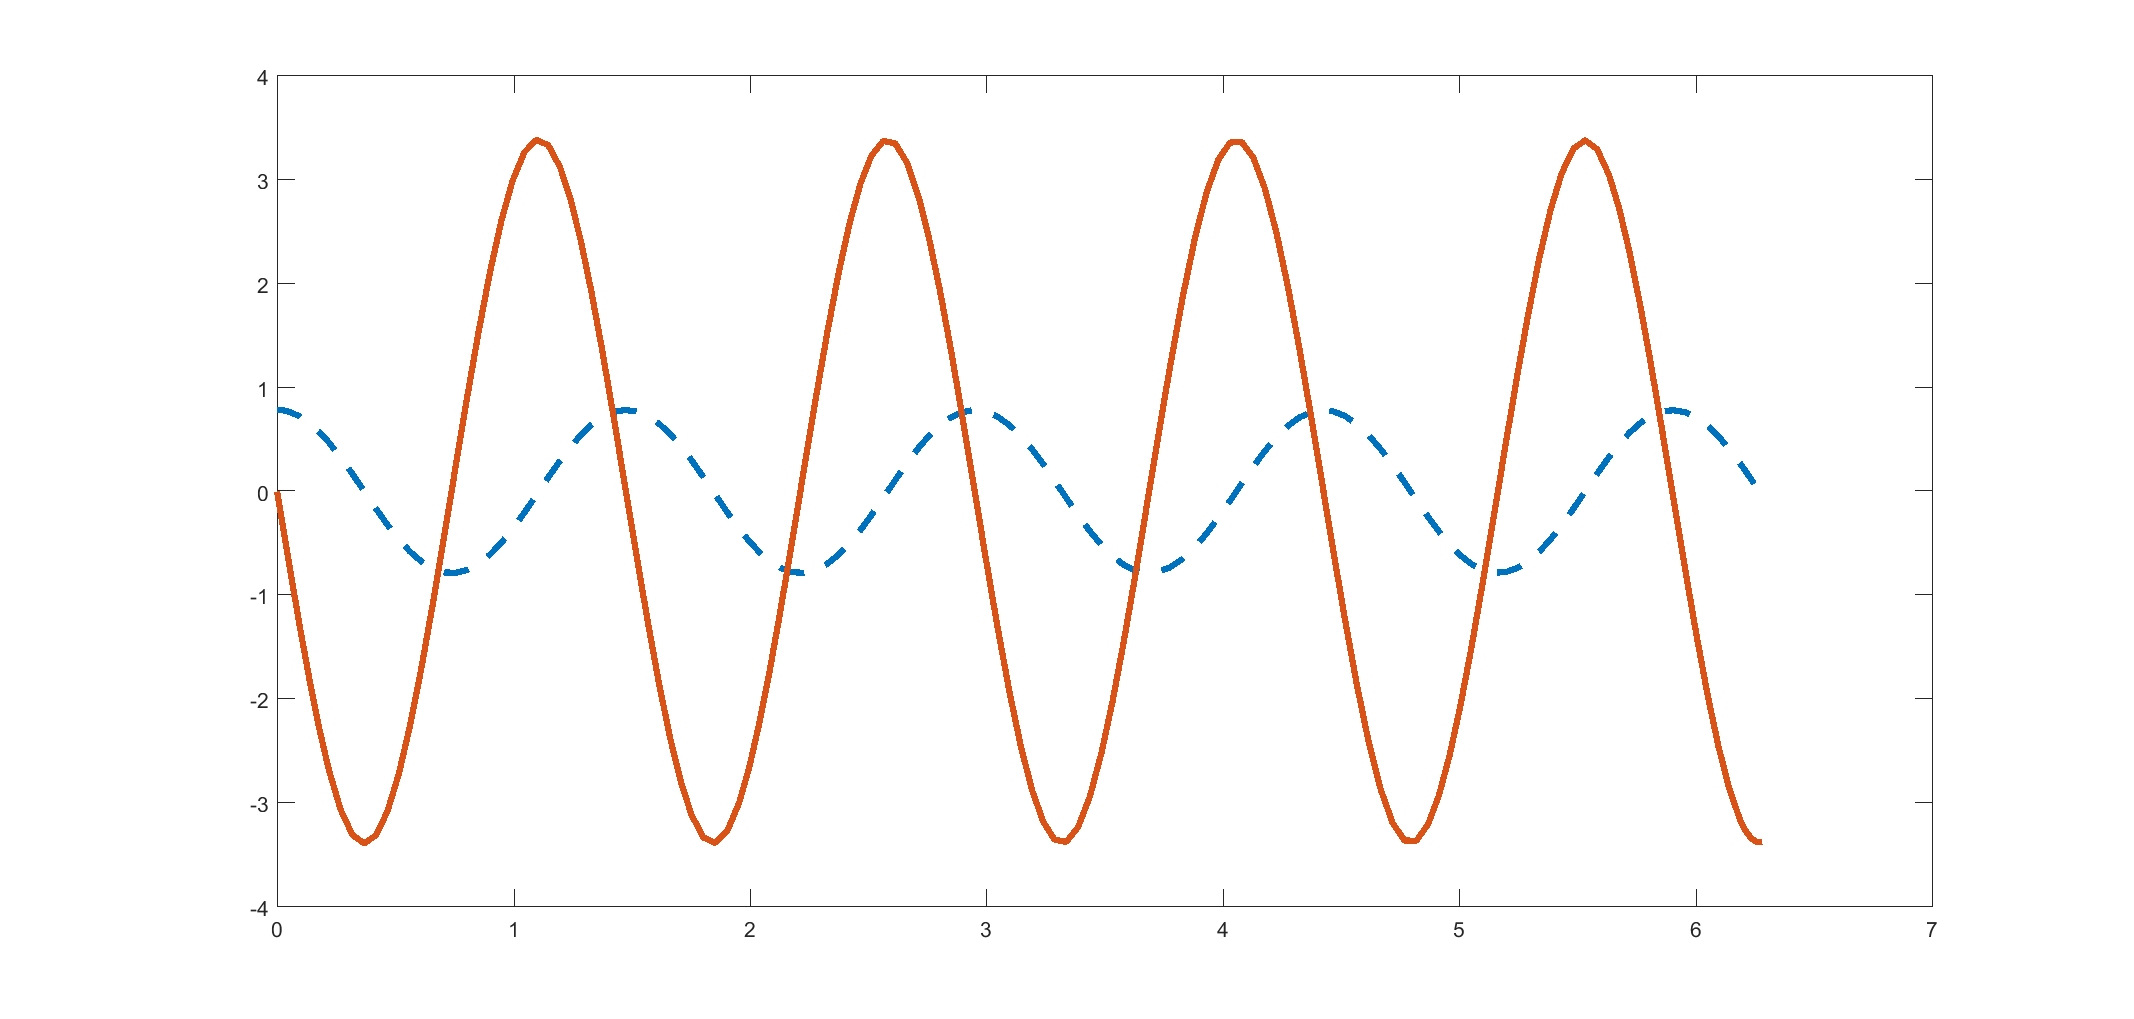
\includegraphics[width=0.75\textwidth]{./img/p14.jpg}
\end{center}
contiene la soluci\'on num\'erica del P.V.I.
$$\begin{array}{rl|}
\theta''+\frac{9.8}{0.5} \,sin(\theta)	&=0\\
\theta(0)	&=\frac{\pi}{4}\\
\theta'(0)	&=0\\ \hline
\end{array}$$
calculada por \texttt{ode45()}. C\'ual de las siguientes proposiciones es cierta.
\end{cuerpo}

\begin{multicols}{2}
\begin{alternativas}
{La funci\'on graficada con una l\'inea s\'olida es $\theta'$.}
{La funci\'on graficada con una l\'inea s\'olida es $\theta$.}
{La funci\'on graficada con una l\'inea intermitente es $\theta'$.}
{La funci\'on graficada con una l\'inea intermitente es $\theta+\theta'$.}
\end{alternativas}
\end{multicols}
\justificacion{0cm}
\end{pregunta}